\subsection{Ma trận tương quan Pearson}

Ở đây ta sử dụng hệ số tương quan - là một chỉ số thống kê đo lường mối liên hệ tương quan giữa hai biến số như Pixel\_Rate và Core\_Speed. Hệ số tương quan có giá trị từ -1 đến 1. Hệ số tương quan bằng 0 (hay gần 0) có nghĩa là hai biến số không có liên hệ gì với nhau, ngược lại nếu hệ số bằng -1 hay 1 có nghĩa là hai biến số có một mối liên hệ tuyệt đối. Nếu giá trị của hệ số tương quan là âm, có nghĩa là khi x tăng cao thì y giảm và ngược lại, khi x giảm thì y tăng. Nếu hệ số tương quan là dương, nghĩa là khi x tăng thì y cũng tăng và x giảm thì y cũng giảm.

Hệ số tương quan Pearson:

$$r = \frac{\sum_{i=1}^{n} (x_i - \bar{x})(y_i - \bar{y})}
{\sqrt{\sum_{i=1}^{n} (x_i - \bar{x})^2 \sum_{i=1}^{n} (y_i - \bar{y})^2}}
$$

Trong đó $\bar{x}$ và $\bar{y}$ là giá trị trung bình của biến số x và y.
Ta có thể kiểm định giả thiết hệ số tương quan bằng 0 (hai biến không có liên hệ) bằng hàm cor.test().

Kết quả tương quan Pearson giữa từng biến định lượng với Pixel\_Rate (sau log-transform) được trình bày trong bảng sau:

\begin{longtable}{|l|c|c|}
\hline
\textbf{Biến} & \textbf{Pearson r} & \textbf{P-value} \\
\hline
Core\_Speed    & 0.3726  & $1.808 \times 10^{-28}$ \\
\hline
Memory\_Speed  & 0.3340  & $7.178 \times 10^{-23}$ \\
\hline
ROPs           & 0.9585  & $\approx 0$ \\
\hline
TMUs           & 0.8751  & $1.146 \times 10^{-260}$ \\
\hline
Memory\_Bus    & 0.5714  & $1.994 \times 10^{-72}$ \\
\hline
Memory         & 0.1133  & $1.138 \times 10^{-3}$ \\
\hline
Process        & $-0.3223$ & $2.542 \times 10^{-21}$ \\
\hline
Shader         & 0.0864  & $1.318 \times 10^{-2}$ \\
\hline
\end{longtable}

Như vậy, biến phụ thuộc Pixel\_Rate có quan hệ thống kê với tất cả các biến (p $<$ 0.05). Tuy nhiên với mục tiêu đơn giản hóa mô hình thì ta sẽ chọn những biến có $|r|$ cao nhất là ROPs, TMUs, Memory\_Bus, Core\_Speed và Memory\_Speed. Biến Process có tương quan âm đáng kể ($r = -0.3223$), cho thấy tiến trình sản xuất nhỏ hơn (công nghệ tiên tiến hơn) đi kèm với Pixel\_Rate cao hơn.

\subsubsection{Scatter plot và Scatter matrix}

\begin{figure}[!h]
    \centering
    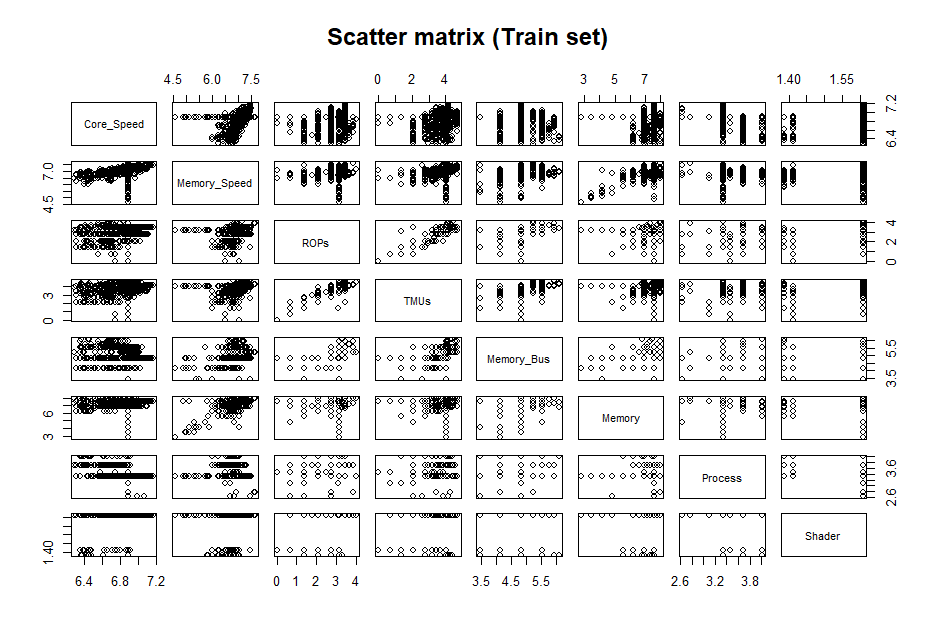
\includegraphics[width=1\linewidth]{images/5.1.png}
    \caption{Scatter matrix toàn bộ biến định lượng trên tập huấn luyện}
    \label{fig:5.1}
\end{figure}

\newpage
Dưới đây là các scatter plot thể hiện mối quan hệ giữa Pixel\_Rate và từng biến định lượng trên tập huấn luyện (sau log-transform). Đường hồi quy màu đỏ thể hiện xu hướng tuyến tính.

\begin{figure}[!h]
    \centering
    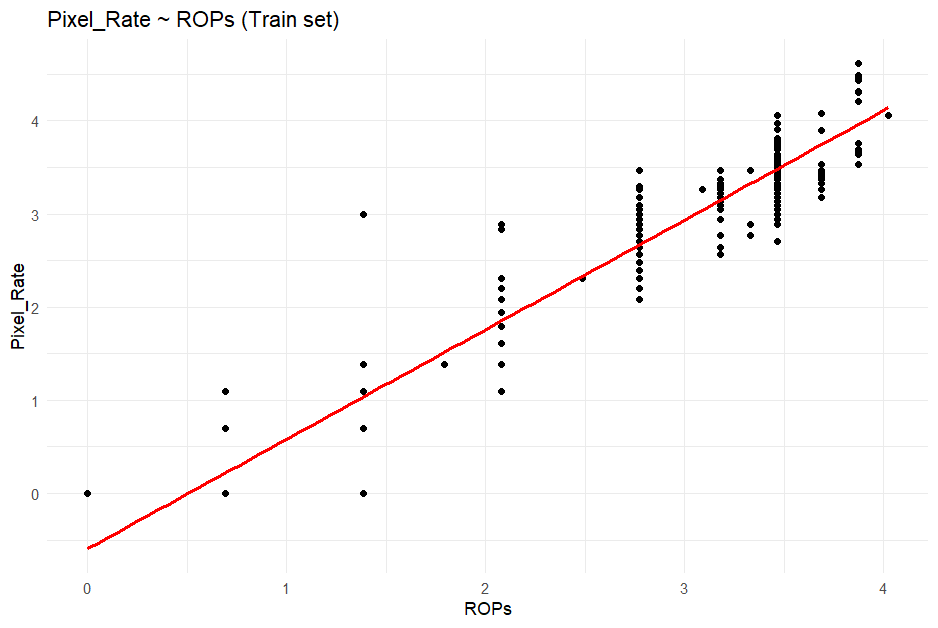
\includegraphics[width=0.85\linewidth]{images/5.4.png}
    \caption{Tương quan Pixel\_Rate $\sim$ ROPs ($r = 0.9585$, tương quan tuyến tính rất mạnh)}
    \label{fig:5.4}
\end{figure}

\begin{figure}[!h]
    \centering
    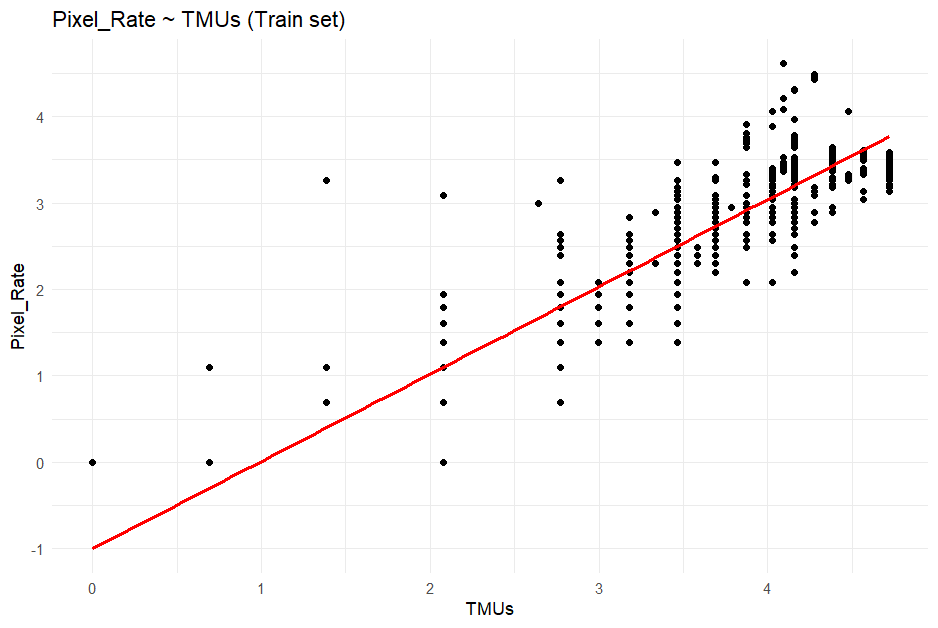
\includegraphics[width=0.85\linewidth]{images/5.5.png}
    \caption{Tương quan Pixel\_Rate $\sim$ TMUs ($r = 0.8751$, tương quan tuyến tính mạnh)}
    \label{fig:5.5}
\end{figure}

\newpage
\begin{figure}[!h]
    \centering
    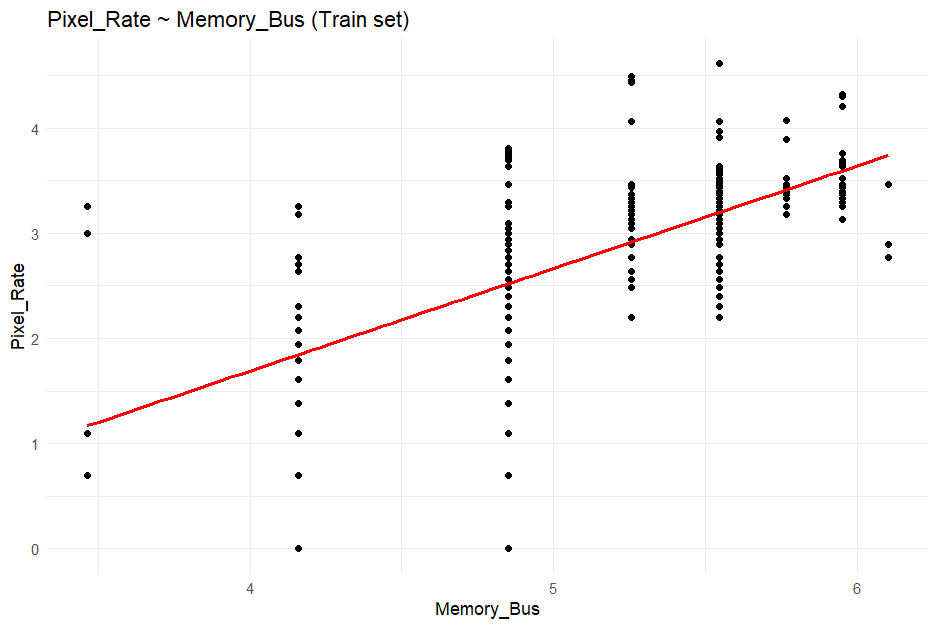
\includegraphics[width=0.85\linewidth]{images/5.6.png}
    \caption{Tương quan Pixel\_Rate $\sim$ Memory\_Bus ($r = 0.5714$, tương quan tuyến tính vừa)}
    \label{fig:5.6}
\end{figure}

\begin{figure}[!h]
    \centering
    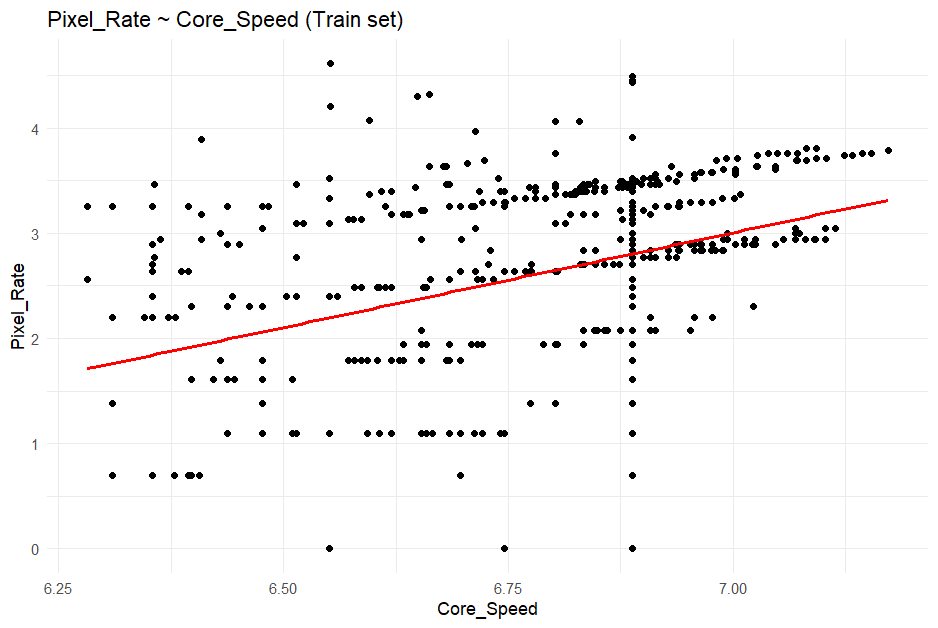
\includegraphics[width=0.85\linewidth]{images/5.2.png}
    \caption{Tương quan Pixel\_Rate $\sim$ Core\_Speed ($r = 0.3726$, tương quan tuyến tính dương)}
    \label{fig:5.2}
\end{figure}

\newpage
\begin{figure}[!h]
    \centering
    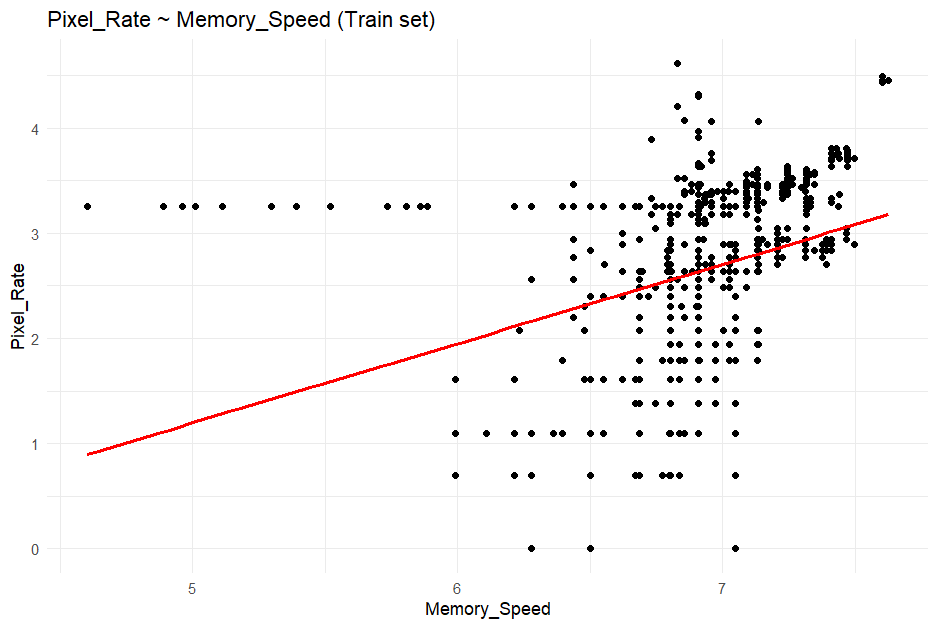
\includegraphics[width=0.85\linewidth]{images/5.3.png}
    \caption{Tương quan Pixel\_Rate $\sim$ Memory\_Speed ($r = 0.3340$, tương quan tuyến tính dương)}
    \label{fig:5.3}
\end{figure}

\begin{figure}[!h]
    \centering
    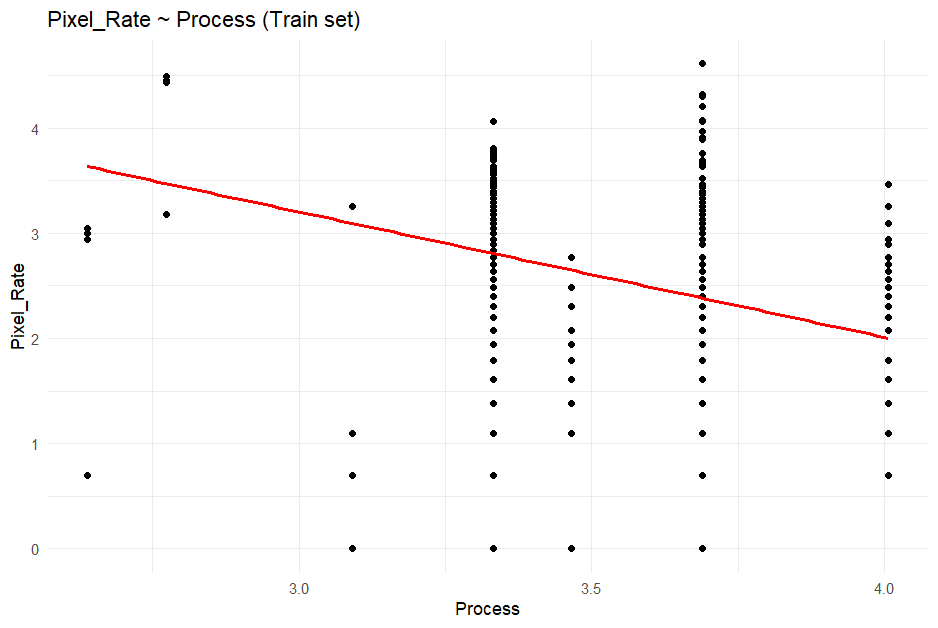
\includegraphics[width=0.85\linewidth]{images/5.8.png}
    \caption{Tương quan Pixel\_Rate $\sim$ Process ($r = -0.3223$, tương quan âm — công nghệ tiên tiến hơn cho Pixel\_Rate cao hơn)}
    \label{fig:5.8}
\end{figure}

\newpage
\begin{figure}[!h]
    \centering
    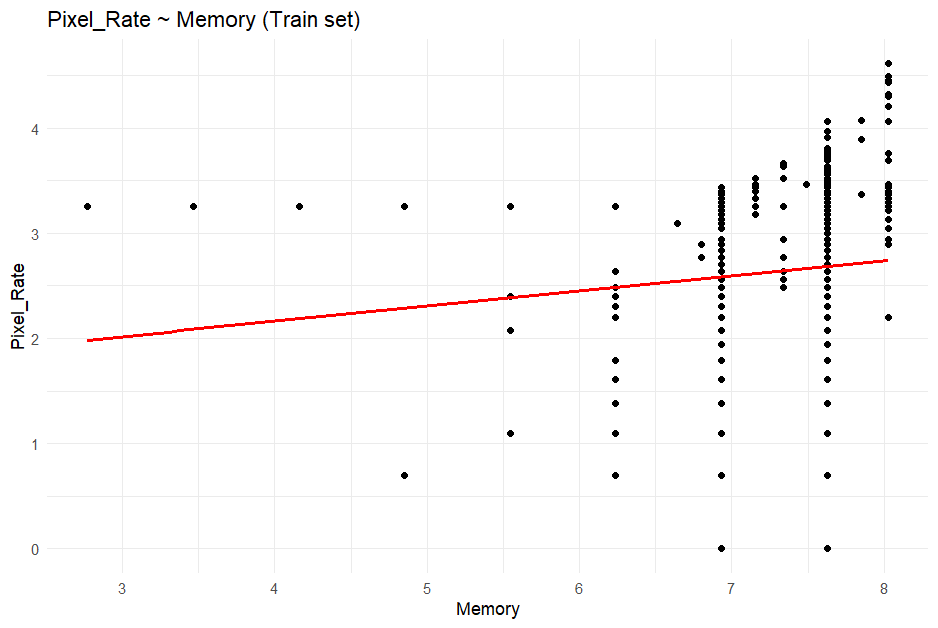
\includegraphics[width=0.85\linewidth]{images/5.7.png}
    \caption{Tương quan Pixel\_Rate $\sim$ Memory ($r = 0.1133$, tương quan yếu)}
    \label{fig:5.7}
\end{figure}

\begin{figure}[!h]
    \centering
    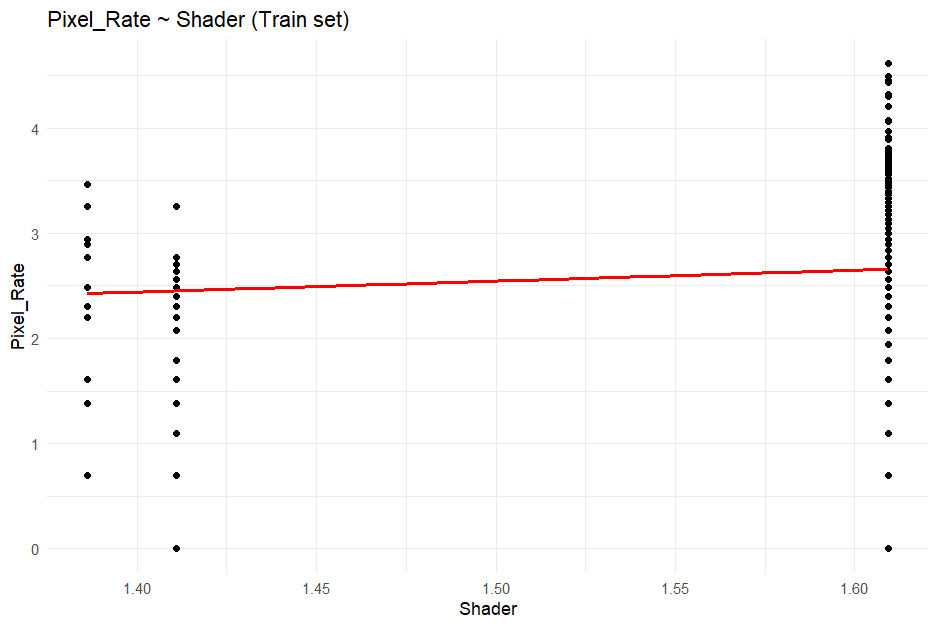
\includegraphics[width=0.85\linewidth]{images/5.9.png}
    \caption{Tương quan Pixel\_Rate $\sim$ Shader ($r = 0.0864$, tương quan rất yếu)}
    \label{fig:5.9}
\end{figure}

\subsection{Phân tích phương sai một yếu tố (ANOVA)}
Nhằm đánh giá sự khác biệt về hiệu suất xử lý đồ họa (Pixel\_Rate) giữa các nhóm phân loại khác nhau. Ta thực hiện phân tích phương sai (ANOVA một chiều) đối với ba biến phân loại chính Manufacturer, Memory\_Type và Resolution\_WxH trên tập huấn luyện (train).

\subsubsection{Mục tiêu}

\begin{itemize}
    \item Kiểm định xem liệu Pixel\_Rate có khác nhau giữa các nhóm phân loại (ví dụ Manufacturer) hay không, ở mức ý nghĩa $\alpha$ = 5\%.
    \item Xác định xem có ít nhất một cặp nhóm có trung bình Pixel\_Rate khác biệt về mặt thống kê.
\end{itemize}

\subsubsection{Bài toán}

\paragraph{Các điều kiện cần kiểm tra trước khi thực hiện ANOVA}

\textbf{Điều kiện 1:} Độc lập của các quan sát

Các giá trị Pixel\_Rate đo được từ mỗi nhóm (Manufacturer / Memory\_Type / Resolution\_WxH) phải được thu thập độc lập.
Kết luận: Do dữ liệu được ghi nhận từ các dòng GPU khác nhau, không có chồng lắp hay phụ thuộc nên điều kiện này được thoả.

\textbf{Điều kiện 2:} Biến phụ thuộc là biến liên tục

Pixel\_Rate là giá trị số thực liên tục (Gpixel/s).
Kết luận: Điều kiện này được thoả.

\textbf{Điều kiện 3:} Phân phối chuẩn trong mỗi nhóm

Dùng kiểm định Shapiro–Wilk trên phần dư hoặc trực tiếp trên từng nhóm.
Nếu $p>0.05$, phần dư (hoặc dữ liệu nhóm) xấp xỉ phân phối chuẩn.

\textbf{Điều kiện 4:} Đồng nhất phương sai giữa các nhóm
Dùng Levene's test.

Nếu $p>0.05$, không bác bỏ giả thiết phương sai bằng nhau.

\paragraph{Giả thuyết của bài toán}
$H_0$: Trung bình Pixel\_Rate của tất cả các nhóm là bằng nhau.
$$H_0: \mu_1 = \mu_2 = \cdots = \mu_k$$

\textbf{Ví dụ với Manufacturer:}

$H_1$: Có ít nhất một cặp nhóm có trung bình Pixel\_Rate khác nhau.
$$H_A: \exists i \neq j \text{ sao cho } \mu_i \neq \mu_j
$$

Sau khi xác nhận (1) - (4), ta tiến hành ANOVA một yếu tố để kiểm định $H_0$ ở mức ý nghĩa $\alpha=0.05$. Nếu $p < 0.05$, bác bỏ $H_0$, kết luận rằng có sự khác biệt về hiệu suất Pixel\_Rate giữa các nhóm.

\subsubsection{Kiểm định giả thuyết}
Trước khi thực hiện phân tích phương sai (ANOVA), hai giả định quan trọng cần được kiểm tra là phân phối chuẩn trong mỗi nhóm (điều kiện 3) và đồng nhất phương sai giữa các nhóm (điều kiện 4). Các kiểm định được sử dụng bao gồm Shapiro-Wilk để đánh giá phân phối chuẩn của phần dư và Levene's test để kiểm tra đồng nhất phương sai. Dưới đây là kết quả kiểm tra cho từng biến phân loại: Manufacturer, Memory\_Type và Resolution\_WxH.

\paragraph{Biến Manufacturer}
\begin{itemize}
    \item \textbf{Kiểm định Shapiro-Wilk (phân phối chuẩn của phần dư):}
    
    \textbf{\textit{Thống kê:}} W = 0.93075
    
    \textbf{\textit{Giá trị:}} $p<2.2 \times10^{-16} $
    
    \textbf{\textit{Kết luận:}} Vì p $<$ 0.05, bác bỏ giả thuyết rằng phần dư tuân theo phân phối chuẩn. Phần dư không xấp xỉ phân phối chuẩn.
    \item \textbf{Kiểm định Levene (đồng nhất phương sai):}
    
    \textit{\textbf{Thống kê:}} F(3, 818) = 5.2397

   \textit{\textbf{Giá trị:}} $p = 1.383 \times10^{-3} $
    
   \textit{\textbf{Kết luận:}} Vì $p < 0.05$, bác bỏ giả thuyết rằng phương sai giữa các nhóm là bằng nhau. Phương sai không đồng nhất.
\end{itemize}

\paragraph{Biến Memory\_Type}
\begin{itemize}
    \item \textbf{Kiểm định Shapiro-Wilk (phân phối chuẩn của phần dư):}
    
    \textbf{\textit{Thống kê:}} W = 0.96471

    \textbf{\textit{Giá trị:}} $p=3.41\cdot{10}^{-13}$
    
    \textbf{\textit{Kết luận:}} Vì p $<$ 0.05, bác bỏ giả thuyết. Phần dư không tuân theo phân phối chuẩn.
    \item \textbf{Kiểm định Levene (đồng nhất phương sai):}
    
    \textbf{\textit{Thống kê:}} F(2, 819) = 27.379
    
   \textbf{\textit{Giá trị:}} $p=3.091\cdot{10}^{-12}$
    
    \textbf{\textit{Kết luận:}} Vì p $<$ 0.05, bác bỏ giả thuyết. Phương sai giữa các nhóm không đồng nhất.
\end{itemize}

\paragraph{Biến Resolution\_WxH}

    \begin{itemize}
        \item \textbf{Kiểm định Shapiro-Wilk (phân phối chuẩn của phần dư):}
        
        \textbf{\textit{Thống kê:}} W = 0.95158
        
        \textbf{\textit{Giá trị:}} $p=8.594\cdot{10}^{-16}$
        
        \textbf{\textit{Kết luận:}} Vì p $<$ 0.05, bác bỏ giả thuyết $H_0$. Phần dư không xấp xỉ phân phối chuẩn.
        \item \textbf{Kiểm định Levene (đồng nhất phương sai):}
        
        \textbf{\textit{Thống kê:}} F(2, 819) = 43.532
        
        \textbf{\textit{Giá trị:}} $p<2.2\cdot{10}^{-16}$
        
        \textbf{\textit{Kết luận:}} Vì p $<$ 0.05, bác bỏ giả thuyết $H_0$. Phương sai giữa các nhóm không đồng nhất.
    \end{itemize}

\newpage
\textbf{Dựa trên phân tích, ta có kết luận:}

Kết quả từ các kiểm định Shapiro-Wilk và Levene cho thấy cả hai giả định về phân phối chuẩn và đồng nhất phương sai đều không được thỏa mãn đối với các biến Manufacturer, Memory\_Type, và Resolution\_WxH (giá trị p $<$ 0.05 trong tất cả các trường hợp). Tuy nhiên, ANOVA vẫn có thể được tiến hành nhờ tính bền vững của phương pháp này với kích thước mẫu lớn $(n \approx 822)$, giúp giảm thiểu tác động của các vi phạm giả định.

\subsubsection{Tiến hành phân tích phương sai và kết quả}
Ta sử dụng hàm aov() trong R để thực hiện phân tích phương sai một yếu tố (ANOVA) cho biến Pixel\_Rate, phân loại theo các biến Manufacturer, Memory\_Type và Resolution\_WxH trên tập dữ liệu huấn luyện (train). Kết quả của mỗi phân tích được in ra bằng hàm summary().

Ta xây dựng mô hình:

\begin{minted}{r}
for (cat in categorical) {
  cat("\nANOVA for", cat, "on Train set\n")
  aov_mod <- aov(as.formula(paste("Pixel_Rate ~", cat)), data = train)
  print(summary(aov_mod))
}
\end{minted}

\textbf{Kết quả phân tích phương sai}

Dưới đây là kết quả ANOVA cho từng biến phân loại:

\paragraph{Biến Manufacturer}

\begin{figure}[!h]
    \centering
    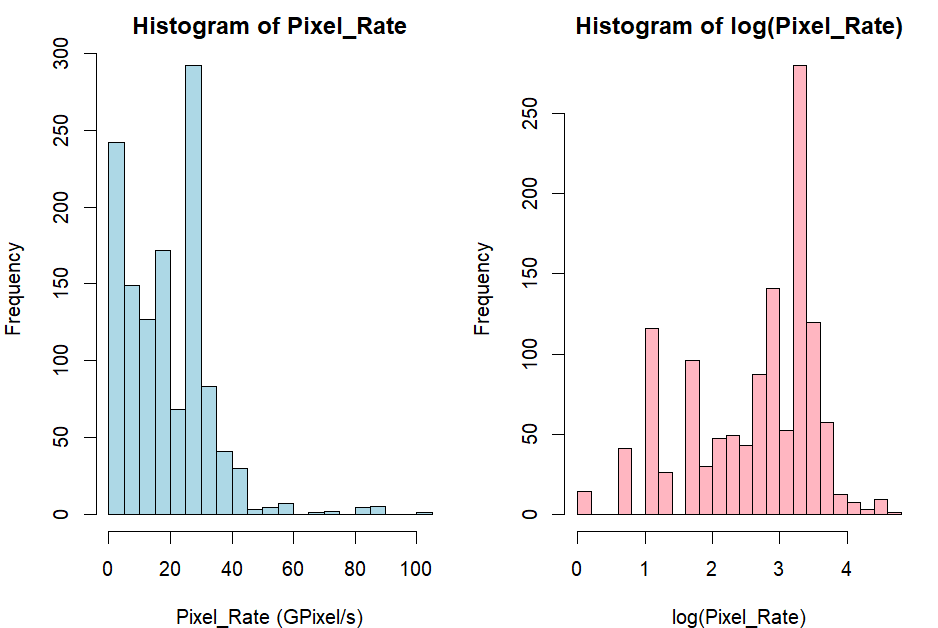
\includegraphics[width=1\linewidth]{images/5.10.png}
    \caption{Boxplot Pixel\_Rate theo Manufacturer (gốc và log-transform)}
    \label{fig:5.10}
\end{figure}

\begin{longtable}{|l|c|c|c|c|c|}
\hline
\textbf{Nguồn biến thiên} & \textbf{Df} & \textbf{Sum Sq} & \textbf{Mean Sq} & \textbf{F value} & \textbf{Pr($>$F)} \\
\hline
Manufacturer & 3 & 27.0 & 8.996 & 11.61 & $1.85 \times 10^{-7}$ *** \\
\hline
Residuals & 818 & 633.6 & 0.775 & & \\
\hline
\end{longtable}

\textbf{Nhận xét:}

Giá trị F = 11.61, cho thấy sự khác biệt về trung bình Pixel\_Rate giữa các nhóm nhà sản xuất.

Giá trị $p = 1.85 \times 10^{-7}$ (nhỏ hơn 0.05), bác bỏ giả thuyết $H_0$ rằng trung bình Pixel\_Rate của các nhà sản xuất là như nhau. Từ boxplot (thang log), ta có thể thấy ATI và Nvidia có trung vị Pixel\_Rate cao hơn AMD và Intel, mặc dù khoảng tứ phân vị khá rộng và chồng lắp nhau.

\paragraph{Biến Memory\_Type}

\begin{figure}[!h]
    \centering
    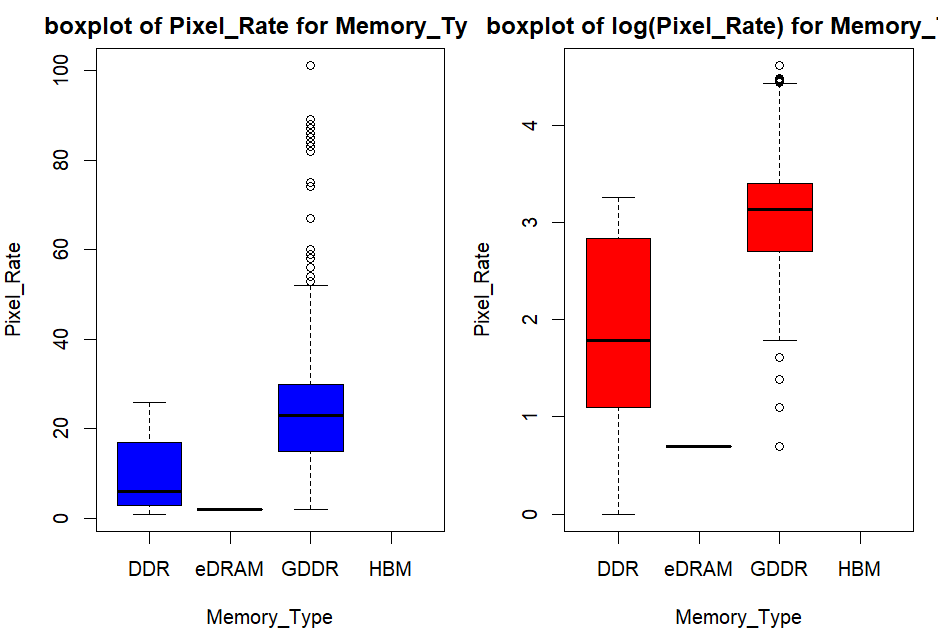
\includegraphics[width=1\linewidth]{images/5.11.png}
    \caption{Boxplot Pixel\_Rate theo Memory\_Type (gốc và log-transform)}
    \label{fig:5.11}
\end{figure}

\begin{longtable}{|l|c|c|c|c|c|}
\hline
\textbf{Nguồn biến thiên} & \textbf{Df} & \textbf{Sum Sq} & \textbf{Mean Sq} & \textbf{F value} & \textbf{Pr($>$F)} \\
\hline
Memory\_Type & 2 & 164.8 & 82.42 & 136.1 & $<2 \times 10^{-16}$ *** \\
\hline
Residuals & 819 & 495.8 & 0.61 & & \\
\hline
\end{longtable}

\textbf{Nhận xét:}

Giá trị F = 136.1 rất cao, cho thấy sự khác biệt đáng kể về trung bình Pixel\_Rate giữa các loại bộ nhớ.

Giá trị $p < 2 \times 10^{-16}$, bác bỏ giả thuyết $H_0$ rằng trung bình Pixel\_Rate của các loại bộ nhớ là như nhau. Boxplot cho thấy GDDR có phân phối Pixel\_Rate rộng và trung vị cao hơn rõ rệt so với DDR và eDRAM.

\paragraph{Biến Resolution\_WxH}

\begin{figure}[!h]
    \centering
    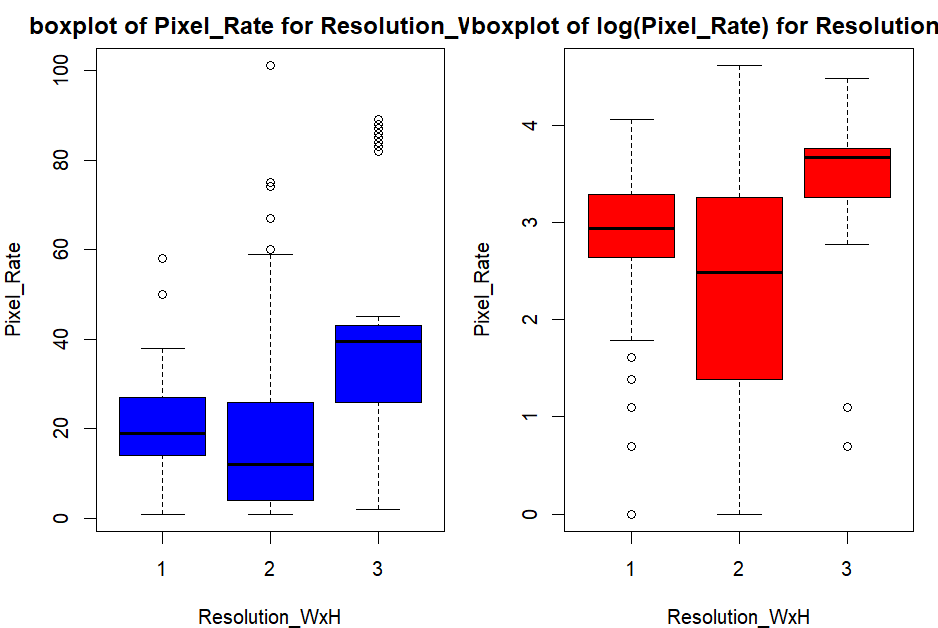
\includegraphics[width=1\linewidth]{images/5.12.png}
    \caption{Boxplot Pixel\_Rate theo Resolution\_WxH (gốc và log-transform)}
    \label{fig:5.12}
\end{figure}

\begin{longtable}{|l|c|c|c|c|c|}
\hline
\textbf{Nguồn biến thiên} & \textbf{Df} & \textbf{Sum Sq} & \textbf{Mean Sq} & \textbf{F value} & \textbf{Pr($>$F)} \\
\hline
Resolution\_WxH & 2 & 76.0 & 38.00 & 53.23 & $<2 \times 10^{-16}$ *** \\
\hline
Residuals & 819 & 584.6 & 0.71 & & \\
\hline
\end{longtable}

\textbf{Nhận xét:}

Giá trị F = 53.23 cao, cho thấy sự khác biệt lớn về trung bình Pixel\_Rate giữa các độ phân giải.

Giá trị $p < 2 \times 10^{-16}$, bác bỏ giả thuyết $H_0$ rằng trung bình Pixel\_Rate của các độ phân giải là như nhau. Boxplot trên thang log cho thấy nhóm 3 (độ phân giải cao nhất) có trung vị Pixel\_Rate vượt trội, trong khi nhóm 2 có trung vị thấp nhất.

\textbf{*Tổng hợp kết quả}

Dưới đây là bảng tổng hợp các giá trị đặc trưng của mô hình ANOVA cho từng biến:

\begin{longtable}{|l|c|c|c|c|}
\hline
\textbf{Biến} & \textbf{Df (giữa nhóm)} & \textbf{Df (trong nhóm)} & \textbf{Sum Sq (SSB)} & \textbf{Sum Sq (SSW)} \\
\hline
Manufacturer & 3 & 818 & 27.0 & 633.6 \\
\hline
Memory\_Type & 2 & 819 & 164.8 & 495.8 \\
\hline
Resolution\_WxH & 2 & 819 & 76.0 & 584.6 \\
\hline
\end{longtable}

\begin{longtable}{|l|c|c|c|c|}
\hline
\textbf{Biến}& \textbf{Mean Sq (MSB)} & \textbf{Mean Sq (MSW)} & \textbf{F value} & \textbf{p-value} \\
\hline
Manufacturer & 8.996 & 0.775 & 11.61 & $1.85 \times 10^{-7}$ \\
\hline
Memory\_Type & 82.42 & 0.610 & 136.1 & $<2\times 10^{-16}$ \\
\hline
Resolution\_WxH & 38.00 & 0.714 & 53.23 & $<2\times 10^{-16}$ \\
\hline
\end{longtable}

\newpage
\textbf{Ghi chú:}
\begin{itemize}
  \item \textbf{\textit{Df (giữa nhóm):}} Bậc tự do giữa các nhóm.
  \item \textbf{\textit{Df (trong nhóm):}} Bậc tự do trong nhóm (Residuals).
  \item \textbf{\textit{Sum Sq (SSB):}} Tổng bình phương giữa các nhóm.
  \item \textbf{\textit{Sum Sq (SSW):}} Tổng bình phương trong nhóm.
  \item \textbf{\textit{Mean Sq (MSB):}} Trung bình bình phương giữa các nhóm.
  \item \textbf{\textit{Mean Sq (MSW):}} Trung bình bình phương trong nhóm.
\end{itemize}

\subsubsection{Kết luận}

Cả ba biến đều có giá trị F cao: 11.61 (Manufacturer), 136.1 (Memory\_Type), 53.23 (Resolution\_WxH) và giá trị p nhỏ hơn rất nhiều so với mức ý nghĩa thống kê $\alpha = 0.05$ (p = $1.85 \times 10^{-7}$ cho Manufacturer; $p < 2 \times 10^{-16}$ cho Memory\_Type và Resolution\_WxH). Điều này cho thấy sự khác biệt rõ rệt về trung bình Pixel\_Rate giữa các nhóm theo từng biến, đồng thời ta bác bỏ giả thuyết $H_0$, kết luận rằng có sự khác biệt có ý nghĩa thống kê về Pixel\_Rate giữa các nhóm trong mỗi biến. Sự khác biệt này có thể xuất phát từ công nghệ sản xuất, chất lượng linh kiện, hoặc đặc điểm thiết kế của từng nhóm. Và để làm rõ hơn về sự khác nhau này, ta sử dụng thêm câu lệnh TukeyHSD và vẽ đồ thị plot().

\subsubsection{Phân tích hậu nghiệm}

Để xác định cụ thể các cặp nhóm nào khác biệt đáng kể, ta tiến hành kiểm định hậu nghiệm Tukey HSD và tính toán effect size ($\eta^2$) nhằm đánh giá mức độ ảnh hưởng của từng biến đến sự biến động của Pixel\_Rate.

Ta sử dụng TukeyHSD(aov\_mod) để hậu nghiệm Tukey, tab[,"Sum Sq"] / sum(tab[ ,"Sum Sq"]) cho tính toán effect size và plot(TukeyHSD(aov\_mod), las = 1) để vẽ đồ thị:

\begin{minted}{r}
for (cat in categorical) {
  cat("\nANOVA for", cat, "on Train set\n")
  aov_mod <- aov(as.formula(paste("Pixel_Rate ~", cat)), data = train)  
  # 6.2 Hậu nghiệm Tukey & Effect size (η²)
  tukey_result <- TukeyHSD(aov_mod)
  print(tukey_result)
  plot(TukeyHSD(aov_mod), las = 1)
  tab <- summary(aov_mod)[[1]]
  eta2 <- tab[,"Sum Sq"] / sum(tab[,"Sum Sq"])
  print(cbind(tab, Eta2 = eta2))
}
\end{minted}

\begin{figure}[!h]
    \centering
    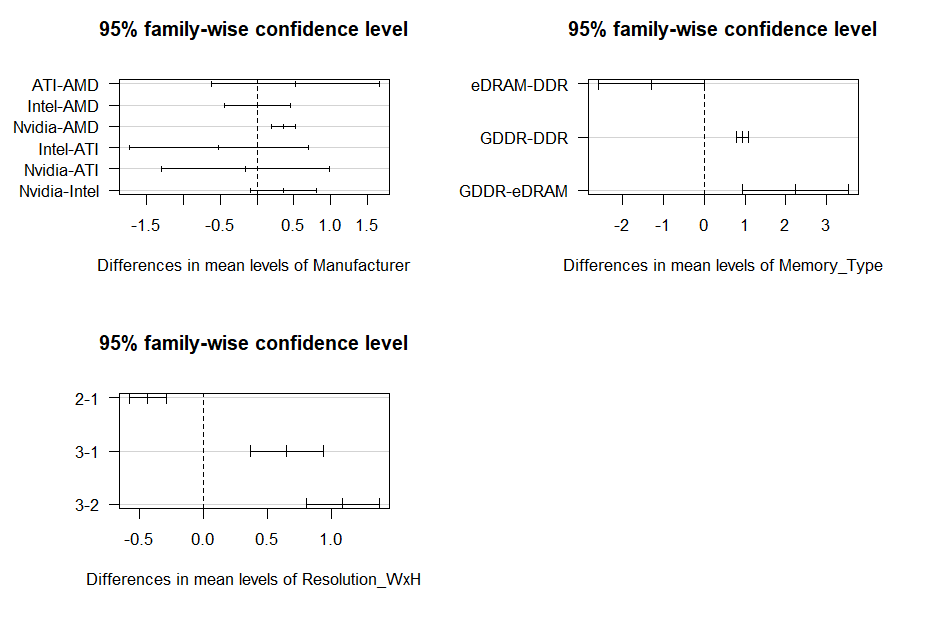
\includegraphics[width=1\linewidth]{images/5.13.png}
    \caption{Đồ thị Tukey HSD cho Manufacturer, Memory\_Type và Resolution\_WxH (mức tin cậy 95\%)}
    \label{fig:5.13}
\end{figure}

Khoảng tin cậy không cắt đường $x = 0$ biểu thị sự khác biệt có ý nghĩa thống kê giữa cặp nhóm tương ứng.

\paragraph{Biến Manufacturer}

\textbf{Kết quả của Tukey HSD:}

\begin{longtable}{|l|c|c|c|c|}
\hline
\textbf{Cặp nhóm} & \textbf{diff} & \textbf{lwr} & \textbf{upr} & \textbf{p adj} \\
\hline
ATI-AMD     & 0.5200  & $-0.6186$ & 1.6586 & 0.6424 \\
\hline
Intel-AMD   & 0.0011  & $-0.4496$ & 0.4518 & 1.0000 \\
\hline
Nvidia-AMD  & 0.3603  &  0.1992  & 0.5214 & 0.0000 \\
\hline
Intel-ATI   & $-0.5190$ & $-1.7328$ & 0.6949 & 0.6893 \\
\hline
Nvidia-ATI  & $-0.1597$ & $-1.2983$ & 0.9789 & 0.9839 \\
\hline
Nvidia-Intel & 0.3592 & $-0.0914$ & 0.8099 & 0.1700 \\
\hline
\end{longtable}

\textbf{Kết quả ANOVA và η²:}

\begin{longtable}{|l|c|c|c|c|c|}
\hline
\textbf{Nguồn} & \textbf{Df} & \textbf{Sum Sq} & \textbf{Mean Sq} & \textbf{F value} & \textbf{$\eta^2$} \\
\hline
Manufacturer & 3 & 26.987 & 8.9956 & 11.613 & 0.04085 \\
\hline
Residuals    & 818 & 633.636 & 0.7746 & & 0.95915 \\
\hline
\end{longtable}

\textbf{Nhận xét:}

Chỉ có cặp \textbf{Nvidia-AMD} có $p\,adj = 0.0000001 < 0.05$, tức là có sự khác biệt đáng kể về Pixel\_Rate giữa Nvidia và AMD. Tất cả các cặp còn lại đều có $p\,adj > 0.05$, không có sự khác biệt đáng kể. Từ đồ thị Tukey HSD, chỉ khoảng tin cậy của Nvidia-AMD không cắt đường $x = 0$, xác nhận kết quả này.
    \begin{itemize}
        \item \textbf{\textit{ATI-AMD:}} diff = 0.5200, khoảng tin cậy $(-0.6186,\ 1.6586)$ bao gồm 0, $p\,adj = 0.6424 > 0.05$ — không đáng kể.
        \item \textbf{\textit{Intel-AMD:}} diff = 0.0011 $\approx 0$, khoảng tin cậy $(-0.4496,\ 0.4518)$ bao gồm 0, $p\,adj = 1.0000$ — không đáng kể.
        \item \textbf{\textit{Nvidia-AMD:}} diff = 0.3603 $> 0$, khoảng tin cậy $(0.1992,\ 0.5214)$ không bao gồm 0, $p\,adj \approx 0$ — Nvidia có Pixel\_Rate trung bình \textbf{cao hơn} AMD $({\bar{x}}_{\text{Nvidia}} > {\bar{x}}_{\text{AMD}})$.
        \item \textbf{\textit{Intel-ATI:}} diff = $-0.5190$, khoảng tin cậy $(-1.7328,\ 0.6949)$ bao gồm 0, $p\,adj = 0.6893 > 0.05$ — không đáng kể.
        \item \textbf{\textit{Nvidia-ATI:}} diff = $-0.1597$, khoảng tin cậy $(-1.2983,\ 0.9789)$ bao gồm 0, $p\,adj = 0.9839 > 0.05$ — không đáng kể.
        \item \textbf{\textit{Nvidia-Intel:}} diff = 0.3592, khoảng tin cậy $(-0.0914,\ 0.8099)$ bao gồm 0, $p\,adj = 0.1700 > 0.05$ — không đáng kể.
    \end{itemize}
    
Từ kết quả trên, chỉ xác định được sự khác biệt thống kê giữa Nvidia và AMD:

\begin{center}
\boxed{\textit{\textbf{Nvidia $>$ AMD (duy nhất có ý nghĩa thống kê)}}}    
\end{center}
    
\textbf{Effect size (η²):} Giá trị η² = 0.04085, cho thấy biến Manufacturer giải thích khoảng 4.09\% sự biến thiên của Pixel\_Rate. Mức ảnh hưởng tương đối nhỏ.

\paragraph{Biến Memory\_Type}

\textbf{Kết quả của Tukey HSD:}

\begin{longtable}{|l|c|c|c|c|}
\hline
\textbf{Cặp nhóm} & \textbf{diff} & \textbf{lwr} & \textbf{upr} & \textbf{p adj} \\
\hline
eDRAM-DDR   & $-1.3039$ & $-2.6005$ & $-0.0072$ & 0.0484 \\
\hline
GDDR-DDR    &  0.9366  &  0.8002  &  1.0730  & 0.0000 \\
\hline
GDDR-eDRAM  &  2.2405  &  0.9464  &  3.5346  & 0.0002 \\
\hline
\end{longtable}

\textbf{Kết quả ANOVA và η²:}

\begin{longtable}{|l|c|c|c|c|c|}
\hline
\textbf{Nguồn} & \textbf{Df} & \textbf{Sum Sq} & \textbf{Mean Sq} & \textbf{F value} & \textbf{$\eta^2$} \\
\hline
Memory\_Type & 2 & 164.831 & 82.4153 & 136.142 & 0.24951 \\
\hline
Residuals    & 819 & 495.792 & 0.6054  & & 0.75049 \\
\hline
\end{longtable}

\textbf{Nhận xét:} Tất cả các cặp đều có $p\,adj < 0.05$ (có sự khác biệt đáng kể). Từ đồ thị Tukey HSD, khoảng tin cậy của cả ba cặp đều không cắt đường $x = 0$.
    \begin{itemize}
        \item \textbf{\textit{eDRAM-DDR:}} diff $= -1.3039 < 0$, khoảng tin cậy $(-2.6005,\ -0.0072)$, $p\,adj = 0.0484$ — eDRAM có Pixel\_Rate trung bình \textbf{thấp hơn} DDR.
        \item \textbf{\textit{GDDR-DDR:}} diff $= 0.9366 > 0$, khoảng tin cậy $(0.8002,\ 1.0730)$, $p\,adj \approx 0$ — GDDR có Pixel\_Rate trung bình \textbf{cao hơn} DDR $({\bar{x}}_{\text{GDDR}} > {\bar{x}}_{\text{DDR}})$.
        \item \textbf{\textit{GDDR-eDRAM:}} diff $= 2.2405 > 0$, khoảng tin cậy $(0.9464,\ 3.5346)$, $p\,adj = 0.0002$ — GDDR có Pixel\_Rate trung bình \textbf{cao hơn} eDRAM $({\bar{x}}_{\text{GDDR}} > {\bar{x}}_{\text{eDRAM}})$.
    \end{itemize}
    
Từ các kết quả trên, thứ tự Pixel\_Rate trung bình là:

\begin{center}
    \boxed{\textbf{\textit{GDDR $>$ DDR $>$ eDRAM}}}
\end{center}

\textbf{Effect size (η²):} Giá trị η² = 0.2495, cho thấy biến Memory\_Type giải thích khoảng 24.95\% sự biến thiên của Pixel\_Rate, mức ảnh hưởng lớn nhất trong ba biến phân loại.

\paragraph{Biến Resolution\_WxH}

\textbf{Kết quả của Tukey HSD:}

\begin{longtable}{|l|c|c|c|c|}
\hline
\textbf{Cặp nhóm} & \textbf{diff} & \textbf{lwr} & \textbf{upr} & \textbf{p adj} \\
\hline
2-1 & $-0.4366$ & $-0.5799$ & $-0.2932$ & 0.0000 \\
\hline
3-1 &  0.6508  &  0.3641  &  0.9376  & 0.0000 \\
\hline
3-2 &  1.0874  &  0.8020  &  1.3728  & 0.0000 \\
\hline
\end{longtable}

\textbf{Kết quả ANOVA và η²:}

\begin{longtable}{|l|c|c|c|c|c|}
\hline
\textbf{Nguồn} & \textbf{Df} & \textbf{Sum Sq} & \textbf{Mean Sq} & \textbf{F value} & \textbf{$\eta^2$} \\
\hline
Resolution\_WxH & 2 & 75.995 & 37.9974 & 53.230 & 0.11504 \\
\hline
Residuals       & 819 & 584.628 & 0.7138  & & 0.88496 \\
\hline
\end{longtable}

\textbf{Nhận xét:}

Tất cả các cặp đều có $p\,adj = 0 < 0.05$, cho thấy có sự khác biệt đáng kể giữa các nhóm. Từ đồ thị Tukey HSD và boxplot, nhóm 3 (độ phân giải cao nhất) nổi bật với Pixel\_Rate trung bình vượt trội.
    \begin{itemize}
        \item \textbf{\textit{2-1:}} diff $= -0.4366 < 0$, khoảng tin cậy $(-0.5799,\ -0.2932)$ — nhóm 2 có Pixel\_Rate trung bình \textbf{thấp hơn} nhóm 1 $({\bar{x}}\_2 < {\bar{x}}\_1)$.
        \item \textbf{\textit{3-1:}} diff $= 0.6508 > 0$, khoảng tin cậy $(0.3641,\ 0.9376)$ — nhóm 3 có Pixel\_Rate trung bình \textbf{cao hơn} nhóm 1 $({\bar{x}}\_3 > {\bar{x}}\_1)$.
        \item \textbf{\textit{3-2:}} diff $= 1.0874 > 0$, khoảng tin cậy $(0.8020,\ 1.3728)$ — nhóm 3 có Pixel\_Rate trung bình \textbf{cao hơn} nhóm 2 $({\bar{x}}\_3 > {\bar{x}}\_2)$.
    \end{itemize}
    
Từ các kết quả trên, thứ tự Pixel\_Rate trung bình là:
\begin{center}
    \boxed{\textbf{\textit{Resolution 3 $>$ Resolution 1 $>$ Resolution 2}}}
\end{center}

\textbf{Effect size (η²):} Giá trị η² = 0.1150, cho thấy biến Resolution\_WxH giải thích khoảng 11.50\% sự biến thiên của Pixel\_Rate, mức ảnh hưởng đáng kể.

\paragraph{Kết luận phân tích hậu nghiệm}

Kết quả kiểm định hậu nghiệm Tukey HSD và effect size η² cho thấy:
\begin{itemize}
    \item \textbf{Manufacturer:} Chỉ có cặp Nvidia-AMD khác biệt đáng kể về Pixel\_Rate, với Nvidia cao hơn AMD. Giá trị η² = 0.04085 cho thấy biến Manufacturer chỉ giải thích khoảng 4.09\% sự biến thiên của Pixel\_Rate --- mức ảnh hưởng thấp nhất trong ba biến phân loại.
    \item \textbf{Memory\_Type:} Có sự khác biệt đáng kể giữa tất cả các loại bộ nhớ (DDR, eDRAM, GDDR), với GDDR có Pixel\_Rate trung bình cao nhất. Giá trị η² = 0.2495 cho thấy biến Memory\_Type có ảnh hưởng mạnh nhất (24.95\%) đến Pixel\_Rate trong ba biến phân loại.
    \item \textbf{Resolution\_WxH:} Có sự khác biệt đáng kể giữa tất cả các nhóm độ phân giải, với nhóm 3 (độ phân giải cao nhất) có Pixel\_Rate trung bình cao nhất. Giá trị η² = 0.1150 cho thấy biến này có ảnh hưởng đáng kể (11.50\%) đến Pixel\_Rate.
\end{itemize}
    
Phân tích phương sai ANOVA cho thấy có sự khác biệt có ý nghĩa thống kê về Pixel\_Rate giữa các nhóm được chia theo biến Manufacturer (F = 11.61, p = $1.85 \times 10^{-7}$), Memory\_Type (F = 136.1, p $< 2 \times 10^{-16}$), và Resolution\_WxH (F = 53.23, p $< 2 \times 10^{-16}$). Kết quả này có thể được sử dụng để đánh giá tác động của các yếu tố phân loại lên hiệu suất GPU (Pixel\_Rate), từ đó hỗ trợ trong việc xây dựng mô hình hồi quy tuyến tính dự báo về sự phát triển của GPU trong mảng hiệu suất dựng ảnh.
